\documentclass[../main.tex]{subfiles}
\begin{document}
\section{Introduction}
\label{sec:introduction}
\begin{figure}
   
\end{figure}



\begin{figure}
    \begin{subfigure}{.24\textwidth}
        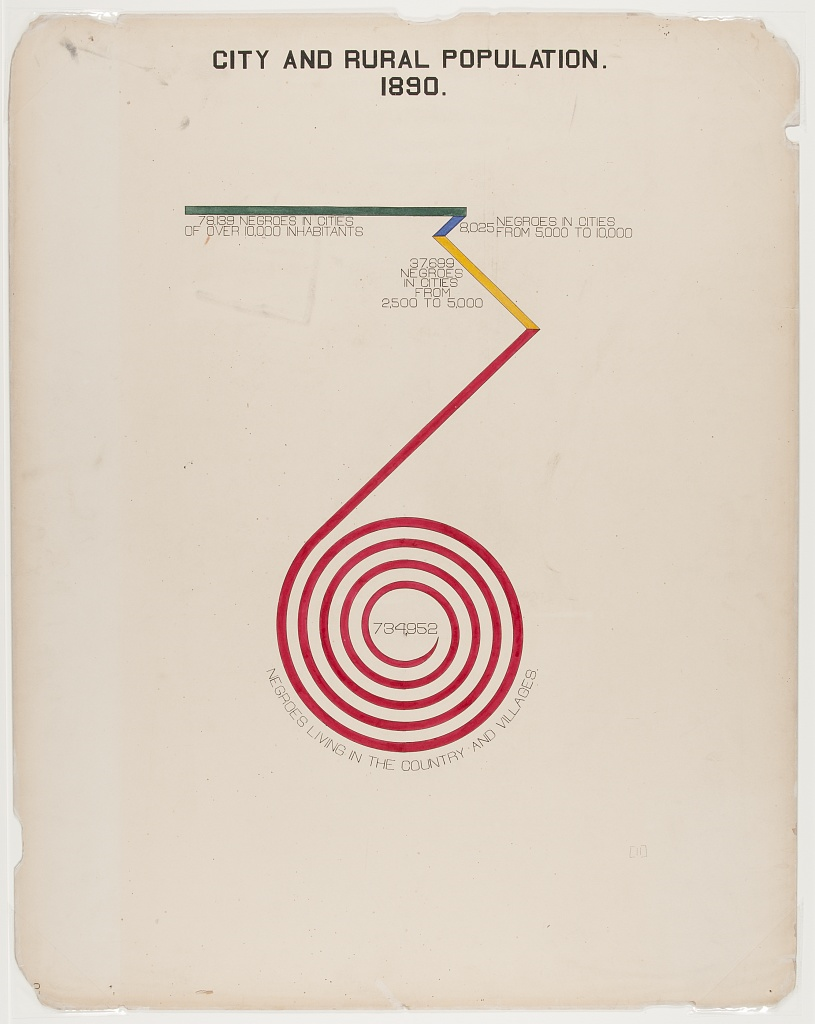
\includegraphics[width=1\textwidth]{figures/intro/du_bois_spinny.png}
        \caption{}
        \label{fig:intro_dpa}
    \end{subfigure}
    \begin{subfigure}{.24\textwidth}
        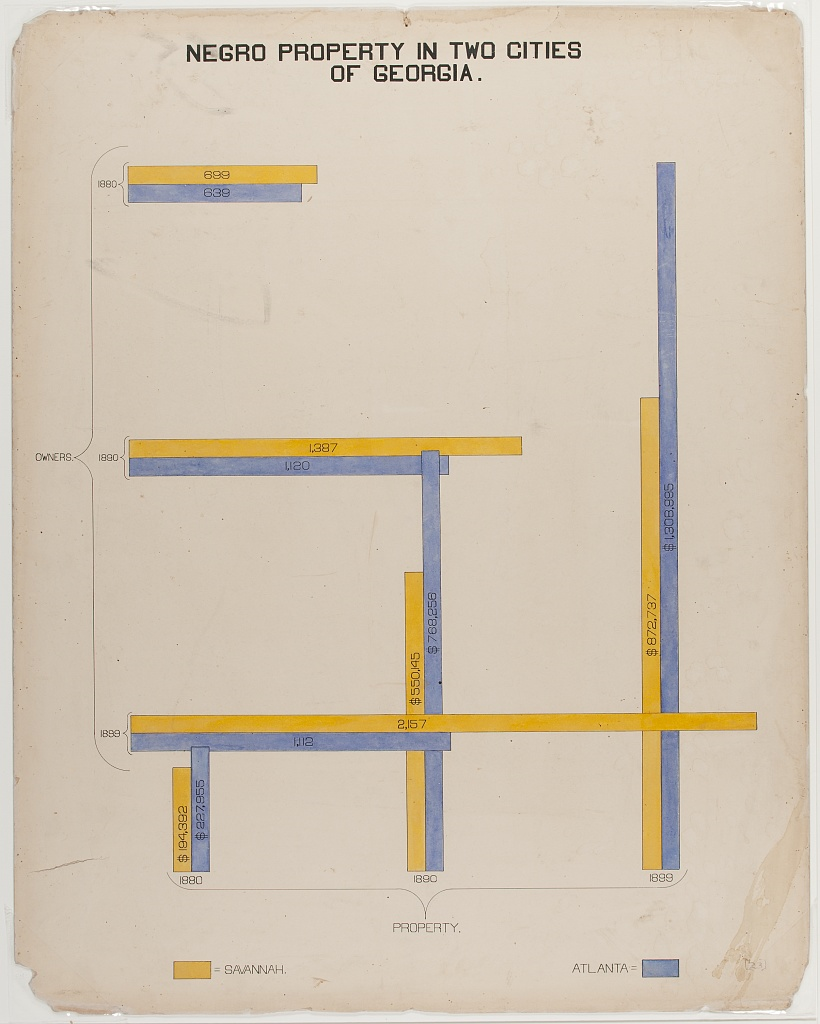
\includegraphics[width=1\textwidth]{figures/intro/du_bois_bar.png}
        \caption{}
        \label{fig:intro_dpb}
    \end{subfigure}
    \begin{subfigure}{.24\textwidth}
        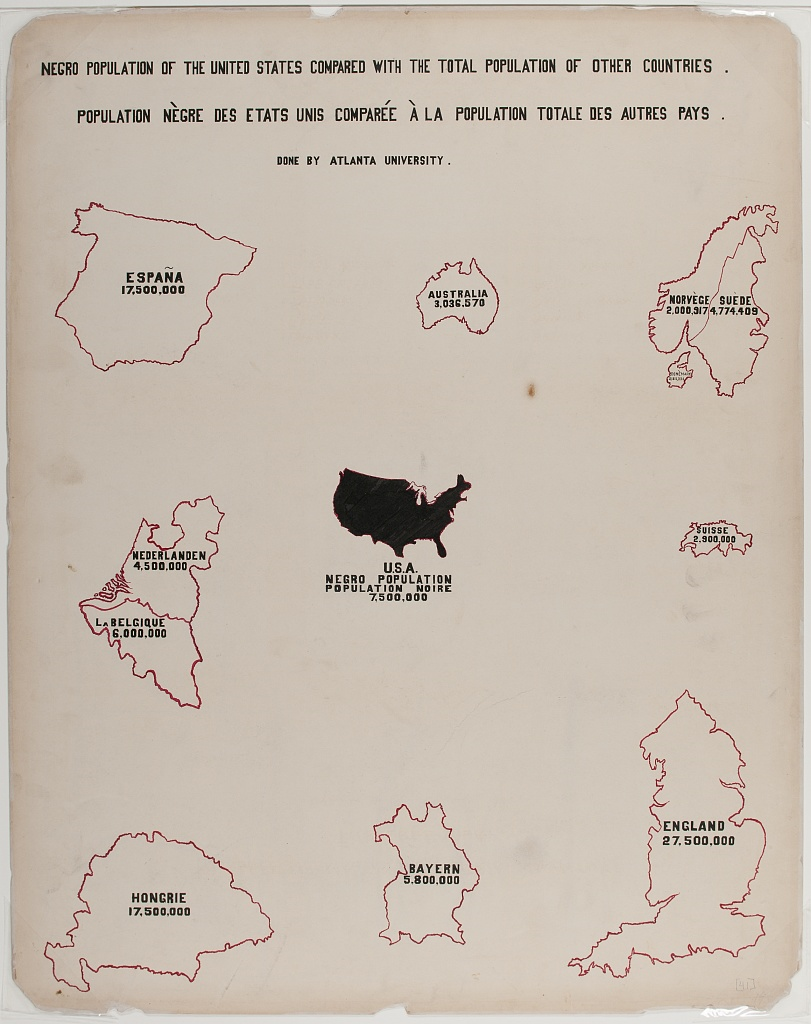
\includegraphics[width=1\textwidth]{figures/intro/du_bois_country.png}
        \caption{}
        \label{fig:intro_dbc}
    \end{subfigure}
    \begin{subfigure}{.24\textwidth}
        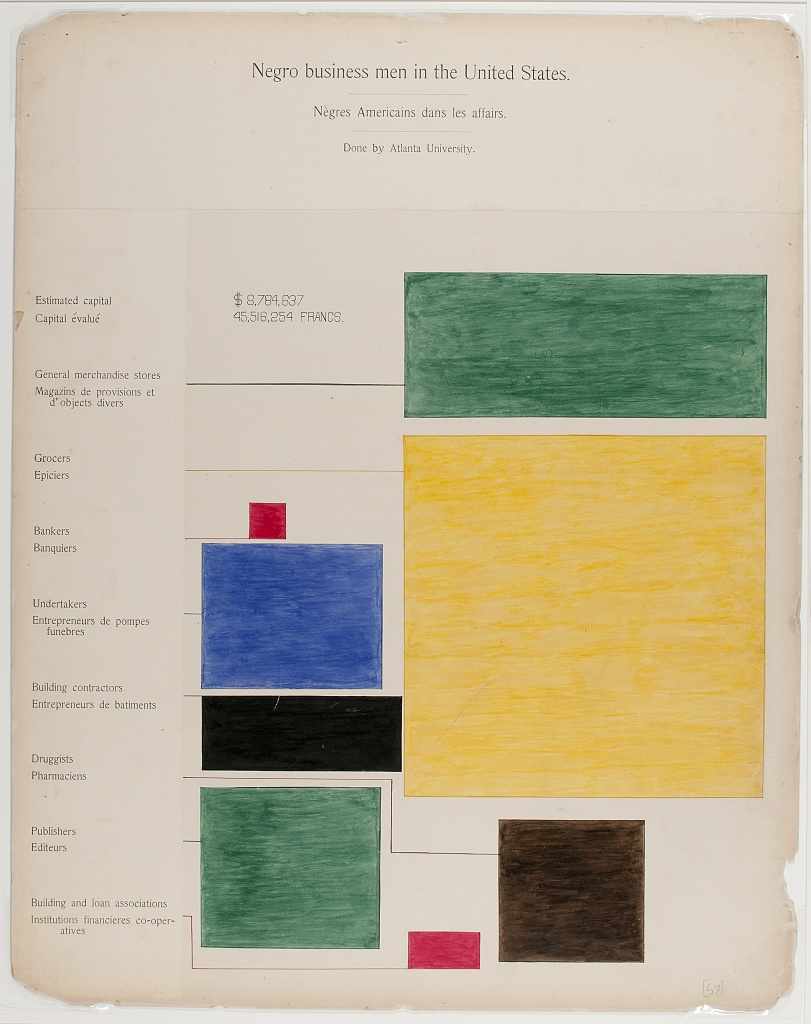
\includegraphics[width=1\textwidth]{figures/intro/du_bois_heat.png}
        \caption{}
        \label{fig:intro_dbd}
    \end{subfigure}
    \caption{Du Bois' data portraits\cite{duboiscenterattheuniversityofmassachusettsBoisDataPortraits2018} of post reconstruction Black American life exemplify that the fundemental characteristics of data visualization is that the visual elements vary in proportion to the source data. In figure~\ref{fig:intro_dpa}, the length of each segment maps to population; in figure~\ref{fig:intro_dpb}, the bar charts are intersected to show the number of property owners and how much they own in a given year; in figure~\ref{fig:intro_dpc} the countries are scaled to population size; and figure~\ref{fig:intro_dpd} is a treemap where the area of the rectangle is representative of the number of businesses in each field. The images here are from the Prints and Photographs collection of the Library of Congress \cite{duboisGeorgiaNegroCity1900, duboisGeorgiaNegroCity1900,duboisSeriesStatisticalCharts,duboisSeriesStatisticalChartsa}}
    \label{fig:intro_dubois}
\end{figure}


\subsection{what is the problem we're trying to solve}
% build better viz libaries
%formally define what constraints on libraries are
% make something seperable and scalable



\subsection{what are we doing}
constraints: toplogy of dataset + structure on the variables
implementation: be fully feature
we can haz compose the things into larger structure. \& has framwework to do larger things w/ algebraic formalizations.



\subsection{What even is a data visualization library?}

Intuitively, data visualizations are drawings where elements of the figure are mapped 
For example, the Du Bois data portraits in figure~\ref{fig:intro_dubois} are not scatter plots or line plots or really maps, but are clearly identifiable as data visualizations because there are some properties of the original data they preserve. 



Mackinlay, expressiveness...Tufte lie principal\cite{mackinlayAutomatingDesignGraphical1986}



"The boundary between scientific visualization and infovis has been explored by Tory and Moller [37] who note ways that discrete and continuous data and the attribute types form a design space that contains both infovis and scientific visualization." \cite{pousmanCasualInformation2007}





Acquired codes of meaning, dubois





\section{Not all data are tables}

Tables, images (Lev), graphs (network X)

set up: dubois

theorists:
bertin, munzner, mackinlay

talk about:
matplotlib arch paper, excel/matlab arch, 
vtk \& ggplot (compare/contrast, we're blending these things) 


\subsection{Terminology}
\textcolor{blue}{Is currently C\&P'ed from my second exam so needs some messaging, but }
\begin{figure}[h!]
%%remake properly at some point
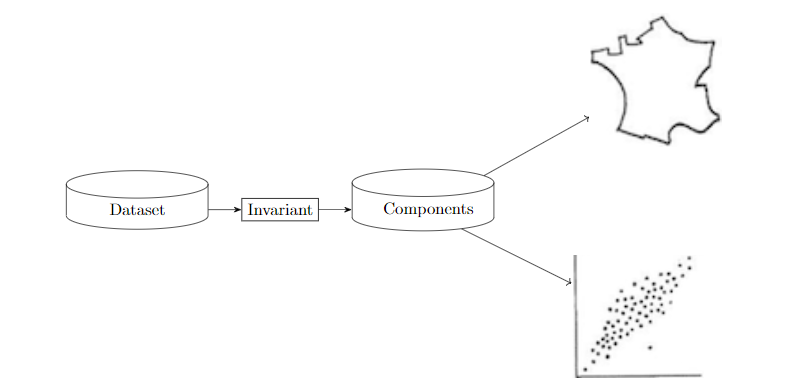
\includegraphics[width=\textwidth]{figures/intro/flowchart.png} 
\caption{To go from a dataset to a visualization, the data is subset based on a set of constraints (the invariant). The resulting subset becomes the components that are visualized, but the choice of visualization is dependent on the type and structure of the component variables.}
\label{fig:flowchart}
\end{figure}

Given a dataset, we need to decide what subset of the data to visualize. Bertin describes the set of constraints used to subset the data as the \textit{invariant}. Formally, the \textit{invariant} is the set of shared characteristics of the data being visualized. When these constraints are applied to the dataset, the resulting subset is what will become the \textit{components} of the visualization \cite{bertinSemiologyGraphicsDiagrams2011a}. 
%%rework this statement for french labor data
%%In figure~\ref{fig:iris_scatter}, the \textit{invariant} common to all the data being visualized is "sepal length", "petal length", and "species" and the \textit{components} are the measurements of these variables. 
As shown in figure~\ref{fig:flowchart}, the final step in creating a visualization is choosing how to encode the
components using retinal (visual) variables.
 

\subsubsection{Retinal (Visual) Variables}
\label{sec:intro_visual_variables}
\begin{figure}[h!]
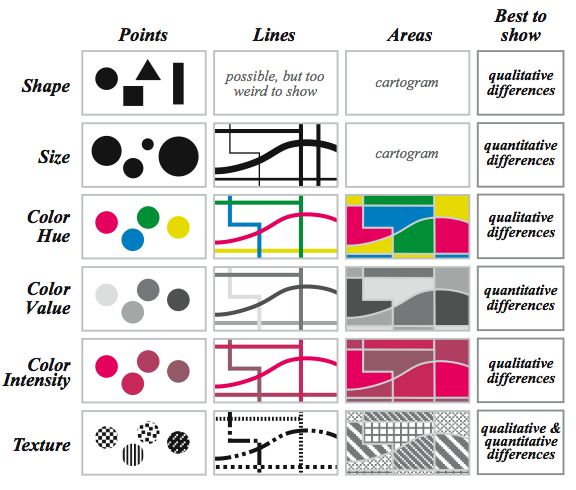
\includegraphics[width=1\textwidth]{figures/intro/retinal_variables.png}
\caption{Retinal variables are a codification of how position, size, shape, color and texture are used to illustrate variations in the \textit{components} of a visualization. This tabular form of Bertin's retinal variables is from Understanding Graphics \cite{malamedInformationDisplayTips2010} who reproduced it from \textit{Making Maps: A Visual Guide to Map Design for GIS} 
\cite{krygierMakingMapsVisual2005}}
\label{fig:retinal_variables}
\end{figure}

Figure~\ref{fig:retinal_variables} illustrates common guidelines for encoding \textit{components}, derived from what Bertin terms a retinal variable and most other visualization theorists call visual variables \cite{bertin_semiology_2011,krygier_making_2005,chambers_graphical_1983,wilkinson_grammar_2005,munzner_visualization_2014}. The columns of figure~\ref{fig:retinal_variables} correspond to the type of observation: discrete points, continuous events (e.g. a timeseries), two dimensional continuous events (e.g. a vector map). The rows of figure~\ref{fig:retinal_variables} describe ways to visualize variations in the \textit{components}; generally, quantitative components are represented by retinal variables that change quantitatively and categorical components are represented by retinal variables that vary qualitatively. In figure~\ref{fig:iris_scatter}, the hue of the marker is used to encode differentiation in species and the position of the marker is used to show variation in petal length and sepal length. The retinal variables suggest that any single visualization is limited to encoding at most about 8 or 9 components. Retinal variables provide guidelines for encoding \textit{components}, but the choice of graph is based on the type and structure of the data. 

\subsubsection{Data Type and Structure}
%% mention tidy/spivak first, set up that we use variable, record, key/index notation
%% define continuity in the math, connectivity in the data
%% topological spaces are frame in terms of continuity
% the implementation of $K$ embeds the connectivity
\label{sec:intro_data_structure}
\begin{figure}[h!]
 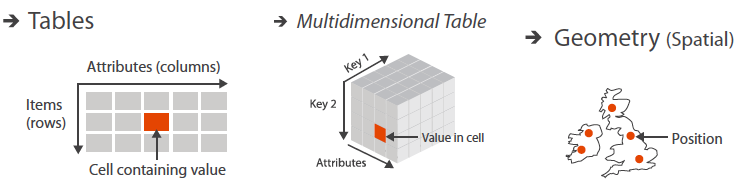
\includegraphics[width=\textwidth]{figures/intro/munzner_datatypes}
\caption{Keys are unique lookup values used to find individual observations in the dataset. Keys are positional references, and can be coordinates on a map or unique values such as a primary key in a database or a (time, latitude, longitude) index in a data cube. Image modified from a diagram from Munzner's \textit{Visualization Analysis and Design} \cite{munznerVisualizationAnalysisDesign2014}}
\label{fig:munzner_datatypes}
\end{figure}

As shown in figure~\ref{fig:flowchart}, there are multiple ways to translate data into pictures. A map is always an option, except when the observations do not have associated coordinates in a physical plane. Tamara Munzner provides a way to distinguish between these datasets using $\{key, value\}$ designations \cite{munznerVisualizationAnalysisDesign2014}. Munzner defines \textit{values} as measurements of interest in the dataset, analogous to dependent variables in statistics. She defines \textit{keys} as indexes that can be used to look up values, analogous to independent variables in statistics and dimensions in computer science. Figure~\ref{fig:munzner_datatypes} illustrates how these keys are used to look up variables in a dataset: 
\begin{itemize}
	\item map: keys are the coordinates of the points
	\item table: row index, database primary key
	\item data cube: row, column, etc. (.e.g. $i,j,k$) index
\end{itemize}

Expanding on Munzner's key and value semantics, in many datasets the keys are discrete variables like time or geophysical locations sampled from a continuous curve, surface, or field. While these observations are discrete samples from the continuous space, often the continuous (functional) characteristic\cite{ramsayFunctionalDataAnalysis2006a,mullerFunctionalVarianceProcesses2006a} of the observational space is also of interest. Besides quantitative discrete, quantitative continuous, or categorical measurement type considerations, the choice of visualization is also influenced by the measurement being on an interval, ratio, nominal, or categorical scale. 

Throughout this form we will be using the following conventions to discuss data:

\begin{description}
    \item[variable]
    \item[index]  
    \item[record]
    \item[value]  
\end{description}

\subsection{how does this tackle the problem? what does it leave on the table?}
% build on butler, gog
% differ from ggplot (d3, vega), vtk, imageJ
%% lets get on the same page about words
% data is topology + variables
% visual variables are sparkly


\subsection{contribution}
 % topological model (abstractions for continuity, formal definition of structure preservation as monoidal action equivarance)
 % prototype

\begin{enumerate}
    \item fiber bundle representation of data and graphics
    \item formalization of variable type structure preservation as monoid action equivariant maps between fibers 
    \item formalization of continuity preservation as equivariant map between base space
    \item algebraic sum for composition of graphics
    \item functional approach to force seperation of scope and concerns
    \item prototype  
\end{enumerate}

\end{document}